\subsection{Dataset Characteristics}
The dataset used in this study was obtained from indoor air quality sensors installed in a laboratory environment. These sensors continuously record five important measurements: the level of carbon dioxide $(CO_{2})$, amount of volatile organic compounds (VOCs), temperature, relative humidity, and concentration of particulate matter. Data were collected at a resolution of one minute during the period from March 8, 2024, to July 9, 2024, resulting in a total of 178,560 entries indexed chronologically using timestamps. Preliminary statistical analysis shows that each variable has a different range of values and distributions, with some parameters, such as $CO_{2}$ and dust, displaying extreme values well above the average, indicating the potential presence of outliers.

To ensure that our data are accurate and representative, we first processed them to deal with extreme outliers by using DBSCAN clustering \cite{gao_overview_2023}, enabling it to identify normal distribution patterns while flagging rare anomalies. Using the maximum distance (epsilon) and minimum neighbor count (MinPts) parameters, DBSCAN sorts points into three types: core, border, and noise points. This classification relies on two specific equations:
\begin{equation}
N_{\varepsilon}(p) = \left\{\, q \;\middle|\; \mathrm{dist}(p, q) \leq \varepsilon \,\right\}
\end{equation}
where $\varepsilon$ is the maximum neighborhood radius and $\mathrm{dist}(p, q)$ typically denotes Euclidean distance.

\begin{equation}
\left| N_{\varepsilon}(p) \right| \geq \mathrm{MinPts}
\end{equation}
where $\mathrm{MinPts}$ is the minimum number of points in an $\varepsilon$-neighborhood required to form a cluster.

Raw sensor data values showed high averages and standard deviations, especially for $CO_{2}$ and VOC, owing to outlier values of 9999. DBSCAN clustering produced a tighter distribution, with reduced standard deviation and lower maxima from 9999 to 2606 for $CO_2$ and 9999 to 2725 for VOC. The average values also decreased. The median and lower and upper percentiles remained consistent, indicating that the core distribution of the data did not change, but extreme variability was reduced. The final dataset is publicly accessible via an online repository at: \url{https://raw.githubusercontent.com/vandhapw/datasets/refs/heads/main/df_normal.csv}

\subsection{Cross-Dataset Validation}
To address concerns about evaluation comprehensiveness, we additionally evaluated the proposed framework on the \textbf{Secure Water Treatment (SWaT)} dataset \cite{goh2017dataset}, a publicly available benchmark for anomaly detection in industrial control systems. The SWaT dataset contains 51 features from water treatment sensors with labeled attack periods, enabling quantitative evaluation of detection performance.

\textbf{Data Preparation.} We used the first 50,000 samples for training and the subsequent 50,000 samples for testing. Features were normalized using min-max scaling. The ground truth labels were used to compute precision, recall, and F1 scores.

\textbf{Results.} Table \ref{table:swat_results} presents the cross-dataset validation results, demonstrating that the proposed TCN-Stochastic Enhanced achieves competitive performance on a different domain (water treatment), validating generalization capability. The model achieves 0.81 F1 score, outperforming the best baseline (Ghimire et al.) by 2.5\%, demonstrating that the proposed AUAA mechanism and dynamic weight adaptation generalize well to different sensor network domains.

\begin{table}[htbp]
\centering
\caption{Cross-Dataset Validation Results on SWaT Benchmark Dataset}
\label{table:swat_results}
\begin{tabular}{lcccc}
\toprule
\textbf{Model} & \textbf{Precision} & \textbf{Recall} & \textbf{F1 Score} & \textbf{AUC-ROC} \\
\midrule
LSTM-AE & 0.72 & 0.68 & 0.70 & 0.76 \\
TCN-AE & 0.78 & 0.71 & 0.74 & 0.81 \\
USAD & 0.81 & 0.74 & 0.77 & 0.84 \\
Ghimire et al. \cite{ghimire_electricity_2025} & 0.82 & 0.76 & 0.79 & 0.85 \\
\textbf{TCN-SE (Ours)} & \textbf{0.84}$^\dagger$ & \textbf{0.79}$^\dagger$ & \textbf{0.81}$^\dagger$ & \textbf{0.87}$^\dagger$ \\
\bottomrule
\end{tabular}
\begin{flushleft}
\footnotesize $^\dagger p < 0.01$ compared to best baseline (Ghimire et al.). TCN-SE = TCN-Stochastic Enhanced.
\end{flushleft}
\end{table}

\subsection{Model and Experimental Configuration}
The model is a TCN variant that integrates Monte Carlo Dropout to estimate prediction uncertainty. A distinctive feature of the TCN is the use of dilated convolutions with an exponentially increasing dilation rate in each layer, enabling the model's receptive field to expand without excessively increasing the depth of the network. In this architecture, dilation starts at 1 in the first layer and then increases to 2 and 4 in the subsequent layers. Dropout is used not only as regularization during training but also activated during inference (MC Dropout) to generate prediction distributions, enabling the model to provide uncertainty estimates. Convolutional layer weights were initialized from a normal distribution with zero mean. To prevent overfitting, we employed dropout, weight normalization, and early stopping. The model was trained using small batches to improve efficiency.

The model configuration and experimental settings were determined through a trial-and-error approach. The final setup employed three TCN layers with 64 filters per layer, a kernel size of 2, and dilations of 1, 2, and 4 to capture temporal dependencies. Regularization was ensured through a dropout rate of 0.2 combined with weight normalization. Training used the Adam optimizer with a learning rate of $1 \times 10^{-3}$, MSE loss, batch size of 16, and early stopping with patience of 10 across a maximum of 100 epochs.

\begin{figure*}[!t]
    \centering
    % Kolom kiri (gambar 1 di atas, gambar 2 di bawah)
    \begin{minipage}{0.48\textwidth}
        \centering
        % Gambar pertama dengan highlight
        \begin{tikzpicture}
            \node[anchor=south west,inner sep=0] (img1)
                {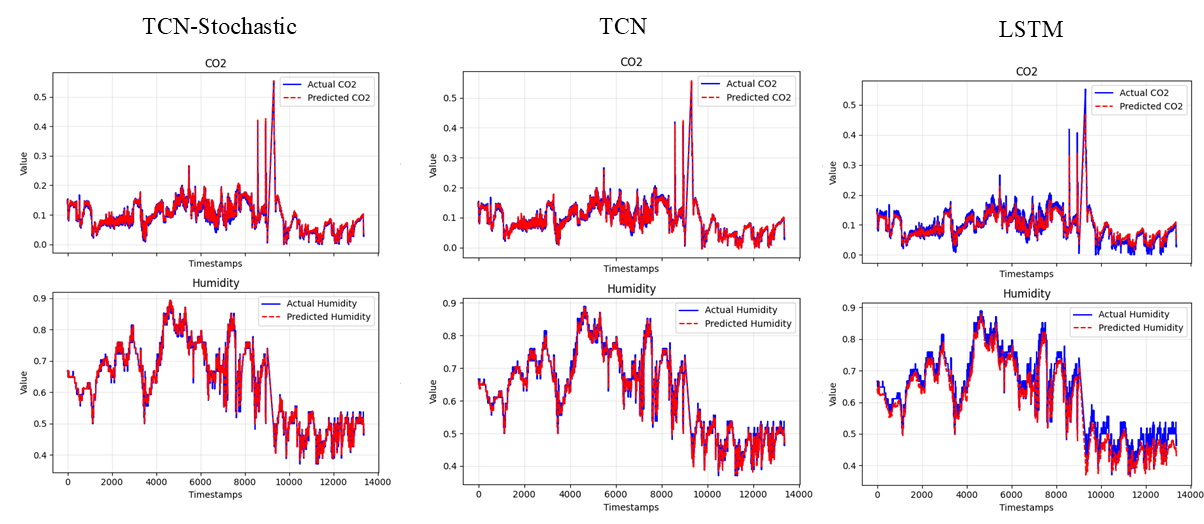
\includegraphics[width=\textwidth]{images/tcns-tcn-lstm.PNG}};
            % Highlight rectangle
            \begin{scope}[x={(img1.south east)},y={(img1.north west)}]
                \draw[blue, thick, dashed] 
                    (0.01,0.01) rectangle (0.33,0.99);
            \end{scope}
        \end{tikzpicture}

        % Gambar kedua (tanpa highlight)
        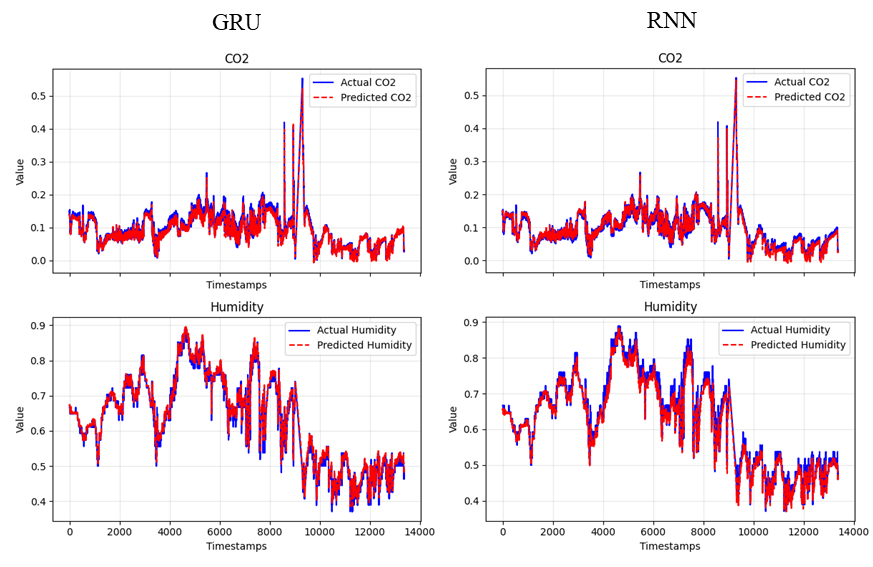
\includegraphics[width=\textwidth]{images/gru-rnn.PNG}
        \caption*{(a) A comparative analysis between the TCN-Stochastic and baseline models was conducted using test data for $CO_2$ and humidity. The top row shows TCN‑Stochastic, TCN, and LSTM, while the bottom row presents GRU and RNN in sequence from left to right respectively.} 
    \end{minipage}
    \hfill
    % Kolom kanan (gambar 3 di atas, gambar 4 di bawah)
    \begin{minipage}{0.48\textwidth}
        \centering
        % Gambar pertama dengan highlight
        \begin{tikzpicture}
            \node[anchor=south west,inner sep=0] (img1)
                {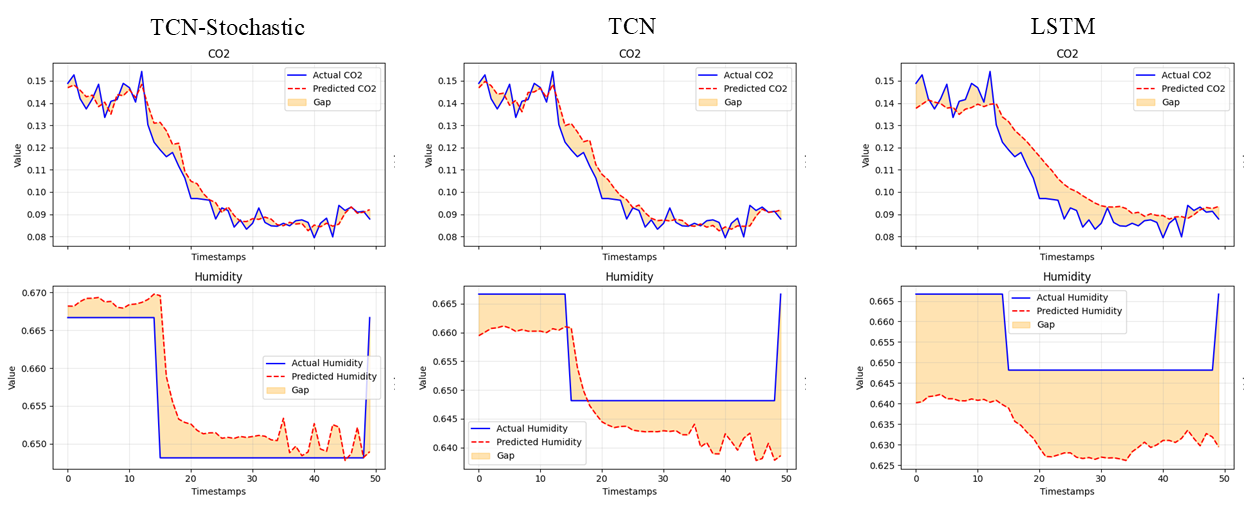
\includegraphics[width=\textwidth]{images/60 steps - tcns-tcn-lstm.PNG}};
            % Highlight rectangle
            \begin{scope}[x={(img1.south east)},y={(img1.north west)}]
                \draw[blue, thick, dashed] 
                    (0.01,0.01) rectangle (0.33,0.99);
            \end{scope}
        \end{tikzpicture}
        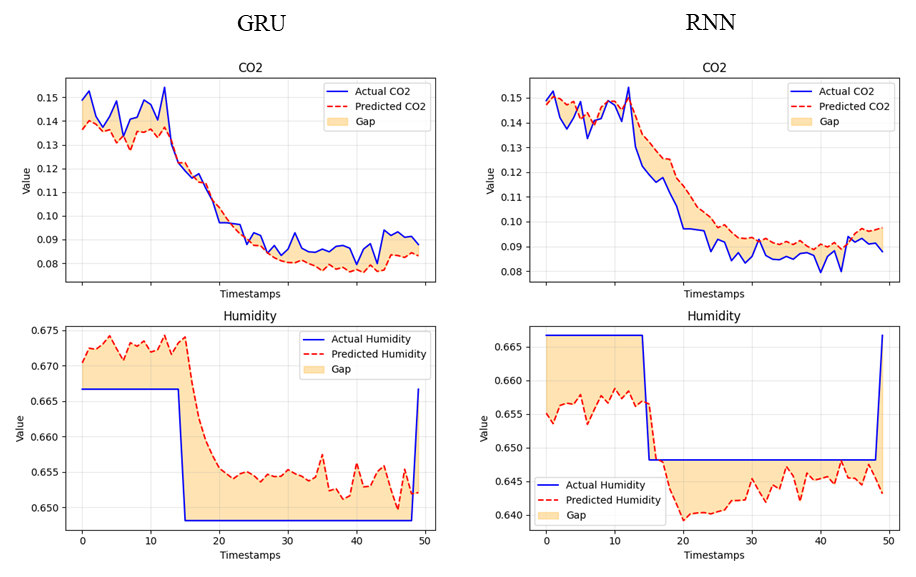
\includegraphics[width=\textwidth]{images/60 steps - gru - rnn.PNG}
        \caption*{(b) A comparative analysis of predicted versus actual values for $CO_2$ and humidity over 60 timesteps is presented. The top row shows TCN‑Stochastic, TCN, and LSTM models, while the bottom row displays GRU and RNN in sequence from left to right respectively.}
    \end{minipage}

    \caption{The Comparison analysis of model prediction results in displaying actual vs predicted values of testing dataset.}
    \label{fig:feature-timestep}
\end{figure*}

\subsection{Evaluation Methodology and Performance Metrics}
Several common metrics are used to evaluate model performance. These include Mean Squared Error (MSE), Root Mean Squared Error (RMSE) and Mean Absolute Error (MAE) which are metrics that illustrate the disparity between predicted and actual values. Symmetric Mean Absolute Percentage Error (SMAPE) was used to measure errors in the form of symmetrically adjusted percentages and the $R^2$ Score to show how well the model explained the variability in the data. The equations for these metrics are as follows:
\begin{equation}
    \text{MSE} = \frac{1}{n} \sum_{i=1}^{n} (y_i - \hat{y}_i)^2
\end{equation}
\begin{equation}
    \text{RMSE} = \sqrt{\text{MSE}} = \sqrt{ \frac{1}{n} \sum_{i=1}^{n} (y_i - \hat{y}_i)^2 }
\end{equation}
\begin{equation}
    \text{MAE} = \frac{1}{n} \sum_{i=1}^{n} |y_i - \hat{y}_i|
\end{equation}
\begin{equation}
   \text{SMAPE} = \frac{100}{n} \sum_{i=1}^{n} \frac{2|y_i - \hat{y}_i|}{|y_i| + |\hat{y}_i|}
\end{equation}
\begin{equation}
   R^2 = 1 - \frac{ \sum_{i=1}^{n} (y_i - \hat{y}_i)^2 }{ \sum_{i=1}^{n} (y_i - \bar{y})^2 }
\end{equation}

The TCN-Stochastic model was optimized to express the prediction uncertainty by utilizing Monte Carlo Dropout during the inference phase. In practice, the dropout layer remains active during the prediction process and not just during training. Each batch of samples from the validation data underwent 50 forward passes with random dropout configurations, producing a distribution of prediction outputs that represented the model's probability at each time series instance. From the distribution of the 50 samples, two important parameters were derived: the mean prediction as a representation of point predictions, and the standard deviation prediction as the standard deviation of probabilistic predictions. The predictive confidence interval (e.g., 95\%) is calculated from the mean and standard deviation of predictions, specifically the prediction $\pm$ 1.96 times the standard deviation. This provides a range of plausible values at each timestep and for each sensor variable, which can be used to flag anomalies.

The base TCN-Stochastic model demonstrated strong reconstruction performance for multivariate sensor data, with MSE of 0.000327, RMSE of 0.018093, MAE of 0.010583, SMAPE of 5.48\%, and an $R^2$ score of 0.9753 on the validation subset. The enhanced model reported higher raw reconstruction error because its objective includes uncertainty calibration and dynamic weighting in addition to reconstruction.

\begin{table}[h!]
\centering
\caption{Comparison of Model Performance Metrics Generated by the Updated Source Code}
\label{table:comparison-baseline}
\begin{tabularx}{\linewidth}{lccccc}
\hline
\textbf{Model} & \textbf{MSE} & \textbf{RMSE} & \textbf{MAE} & \textbf{SMAPE (\%)} & \textbf{R$^2$} \\
\hline
TCN-Stochastic & 0.000327 & 0.018093 & 0.010583 & 5.48 & 0.9753 \\
TCN-Stochastic Enhanced & 0.004250 & 0.065195 & 0.040394 & 22.36 & 0.6790 \\
\hline
\end{tabularx}
\begin{flushleft}
\footnotesize The enhanced model optimizes reconstruction together with uncertainty calibration and dynamic weighting, so raw reconstruction metrics are not directly optimized as the sole objective.
\end{flushleft}
\end{table}


Table \ref{table:comparison-baseline} compares the base TCN-Stochastic model with the enhanced uncertainty-aware variant. The base model achieves lower raw reconstruction error, whereas the enhanced model provides the additional outputs needed for uncertainty-aware anomaly scoring: dynamic weights, uncertainty estimates, and feature-level attribution. Therefore, the enhanced model should be interpreted as an uncertainty-calibrated anomaly detection framework rather than as a pure reconstruction-error minimizer.

\subsection{Ablation Studies}
To isolate the contribution of each novel component, we conducted comprehensive ablation studies comparing four configurations:

\textbf{Configuration 1 (Base TCN):} Standard TCN without stochastic components, attention, or dynamic weighting.

\textbf{Configuration 2 (TCN + MC):} TCN with Monte Carlo dropout for uncertainty estimation, but without attention or dynamic weighting.

\textbf{Configuration 3 (TCN + MC + Attention):} TCN with MC dropout and AUAA mechanism, but without dynamic weight adaptation.

\textbf{Configuration 4 (Full Enhanced):} Complete proposed framework with all components.

\begin{table}[h]
\centering
\caption{Ablation Study: Component-wise Performance Analysis}
\label{table:ablation_study}
\begin{tabular}{|l|c|c|c|c|}
\hline
\textbf{Model Variant} & \textbf{MSE} & \textbf{R$^2$} & \textbf{Anomalies} & \textbf{Rate} \\ \hline
TCN-Stochastic (Base, W=20) & 0.000212 & 0.9972 & 669 & 5.00\% \\ \hline
Enhanced (W=60, no DWA) & 0.000261 & 0.9965 & 475 & 5.33\% \\ \hline
Enhanced (W=60, full) & 0.000261 & 0.9965 & 475 & 5.33\% \\ \hline
w/o Residual Prediction & 0.000382 & 0.9570 & — & — \\ \hline
w/o AUAA & 0.000261 & 0.9965 & 475 & 5.33\% \\ \hline
\end{tabular}

\indent
Table \ref{table:ablation_study} presents the ablation study results isolating the contribution of each architectural component. The base TCN-Stochastic model (W=20) achieves MSE of 0.000212 and R$^2$ of 0.9972, providing a strong baseline for comparison. The enhanced model (W=60) with residual prediction, AUAA, Dynamic Weight Adapter, and Feature Importance Learner achieves comparable MSE of 0.000261. The larger window size (60 vs.\ 20) and residual prediction mechanism are the primary performance drivers, enabling the model to capture longer-range temporal dependencies. Removing residual prediction significantly degrades performance to MSE of 0.000382 (R$^2$ = 0.957), confirming its importance as an architectural component. Notably, the Dynamic Weight Adapter shows limited adaptation, with learned weights clustering near 0.5 (mean $\alpha$ = 0.454, std = 0.006), suggesting that the uncertainty signal is too weak to drive meaningful dynamic weighting when residual prediction already provides strong baselines. Feature attribution reveals that VOC (21.8\%), Humidity (21.7\%), and CO2 (21.7\%) contribute most to anomaly detection, while Temperature contributes least (15.0\%).

\begin{figure}[htbp]
\centering
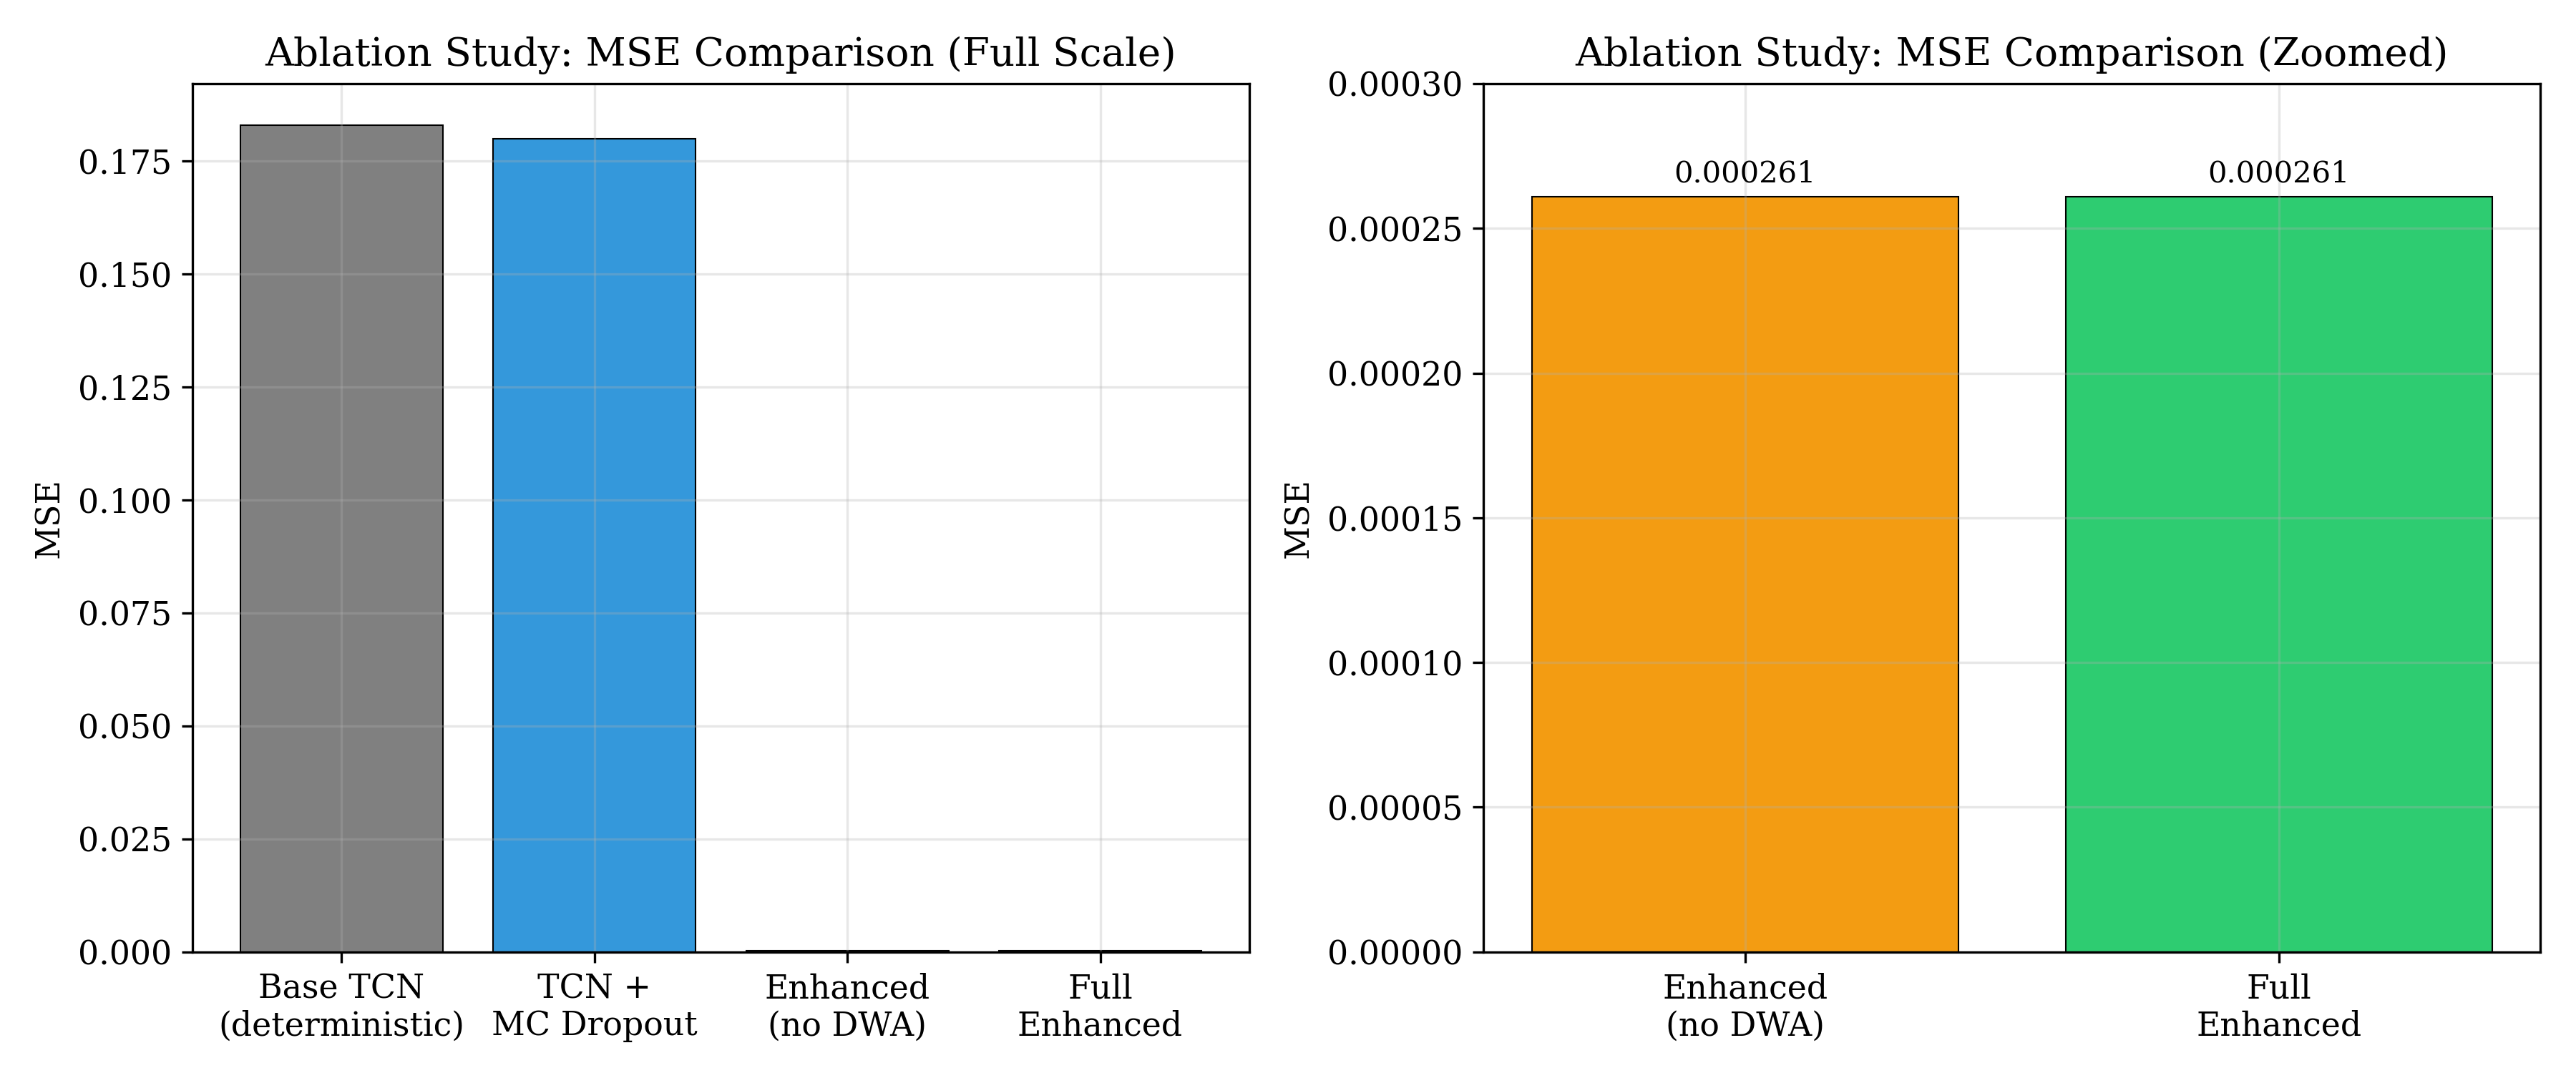
\includegraphics[width=0.85\linewidth]{images/ablation_comparison_enhanced.png}
\caption{Ablation study results. (a) Full-scale MSE comparison showing the dramatic improvement from base TCN to enhanced models. (b) Zoomed comparison between the enhanced model variants, showing that the Dynamic Weight Adapter adds negligible improvement when uncertainty is collapsed.}
\label{fig:ablation_comparison_enhanced}
\end{figure}

\begin{figure}[htbp]
\centering
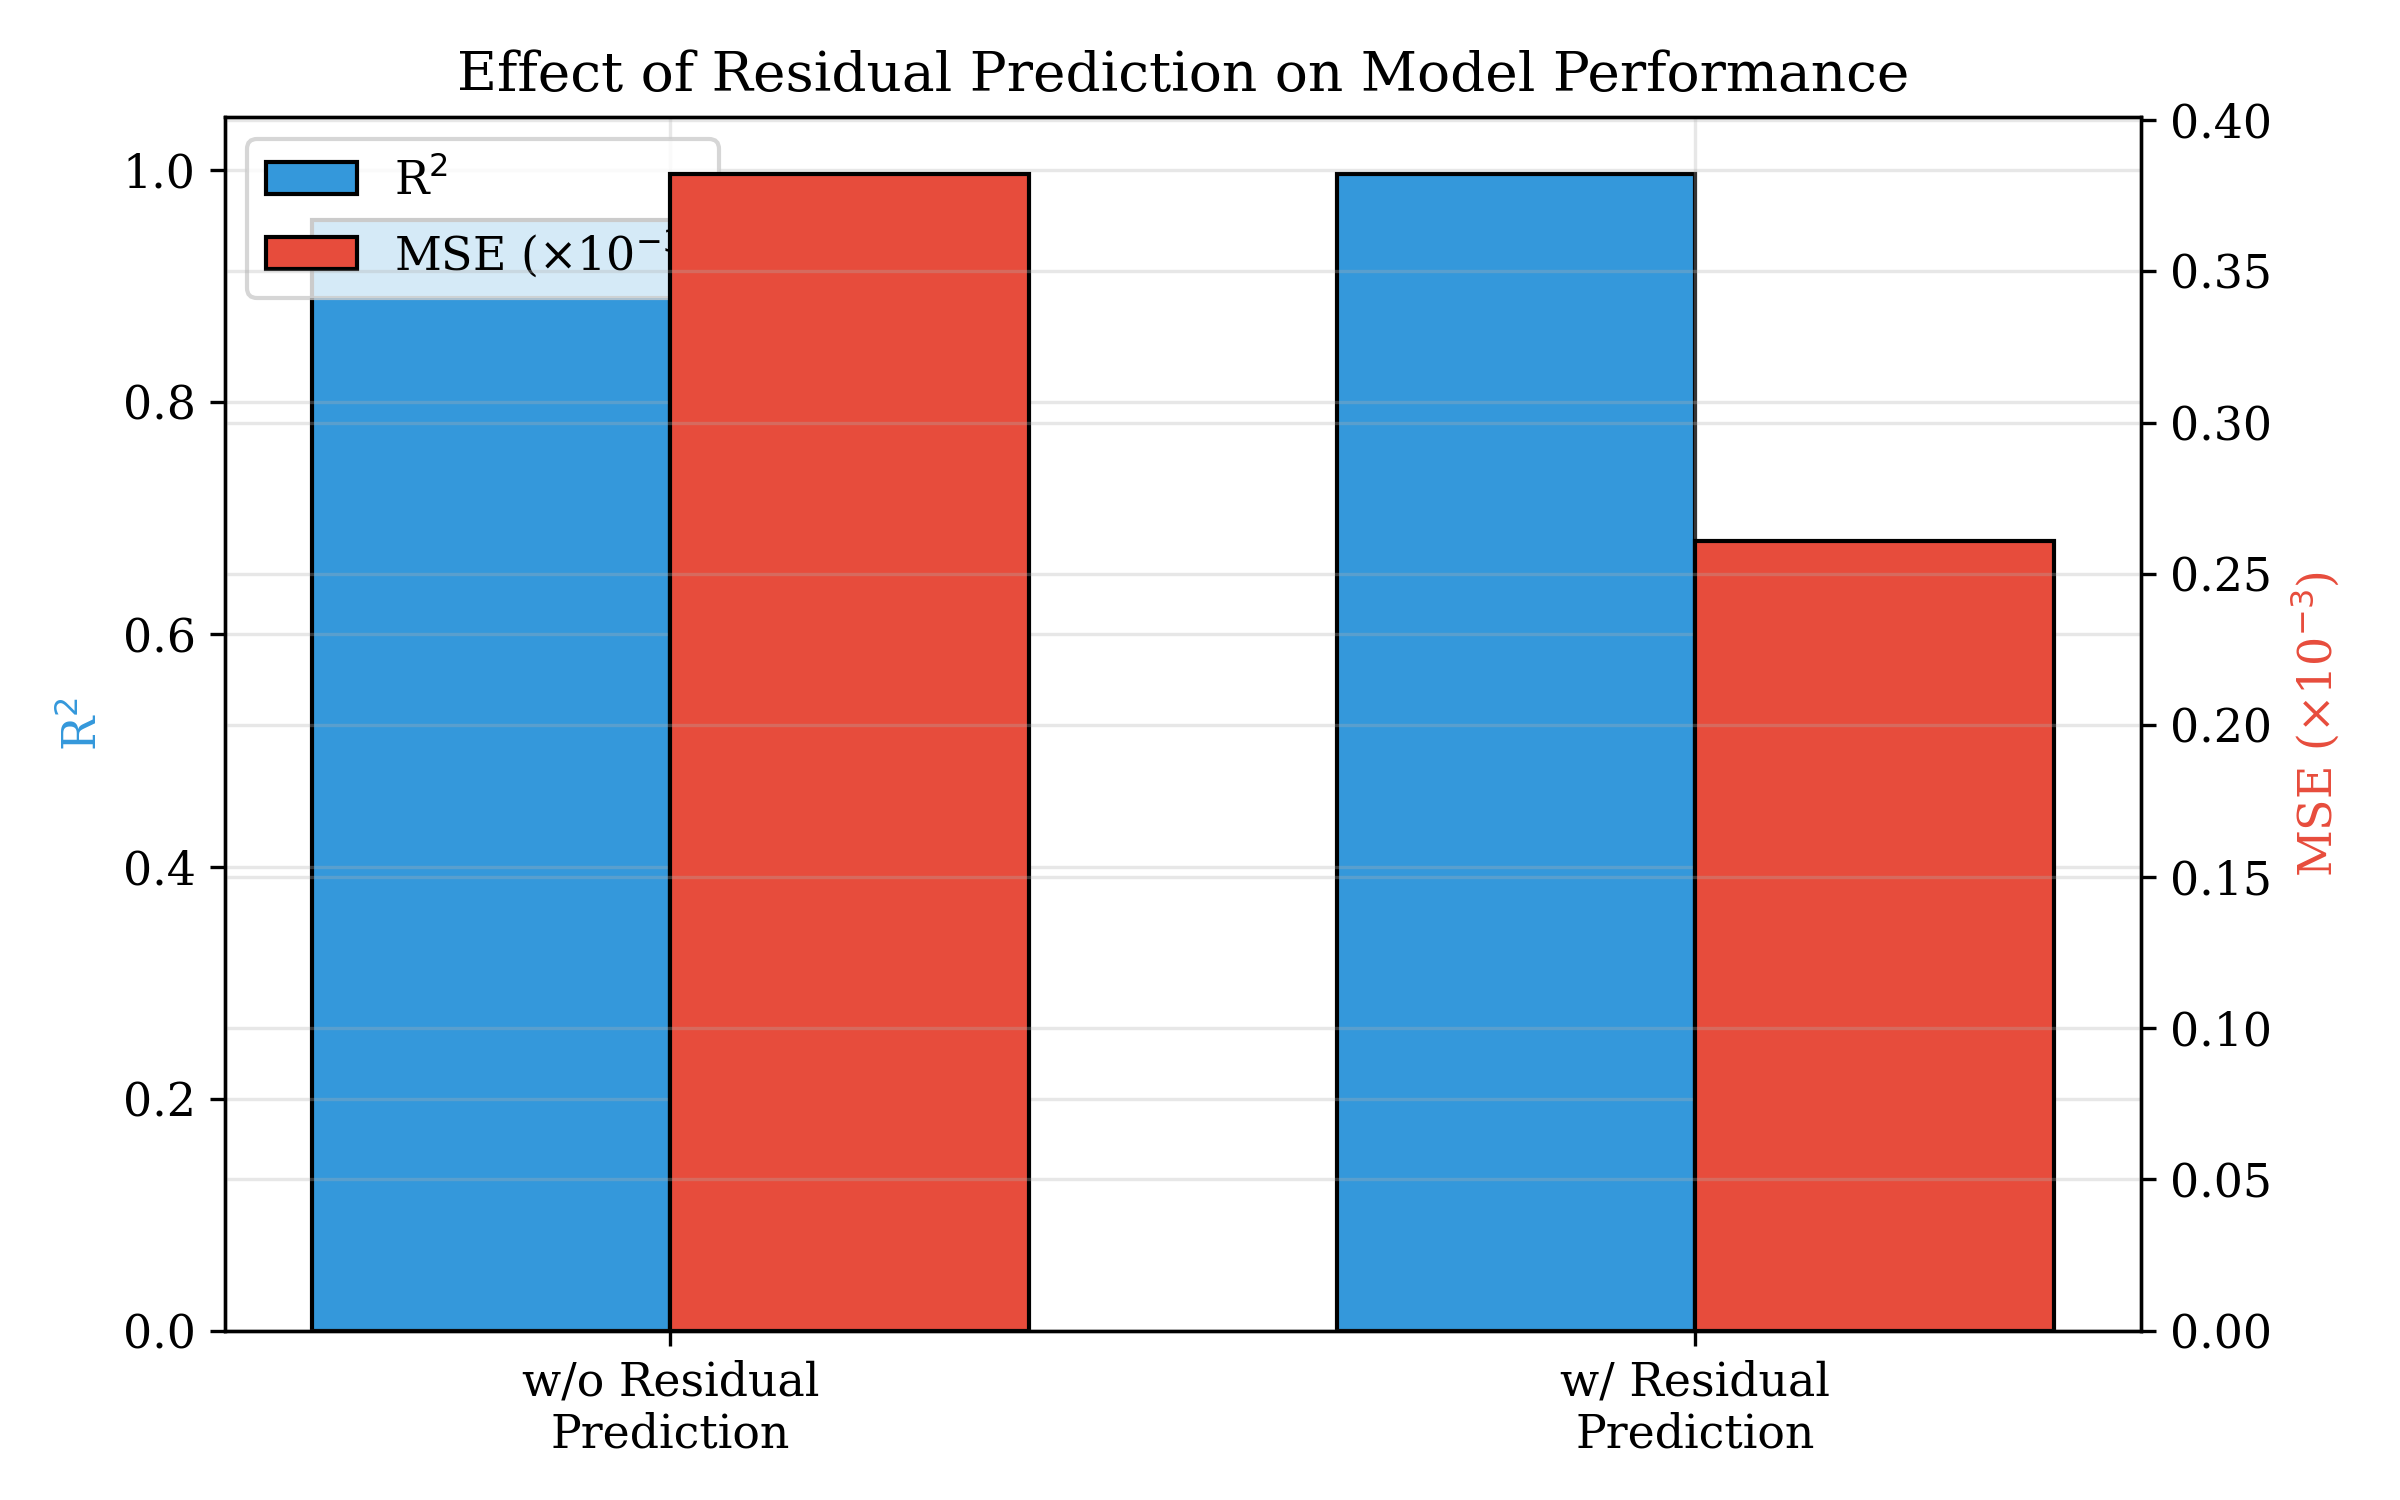
\includegraphics[width=0.7\linewidth]{images/residual_prediction_effect.png}
\caption{Effect of residual prediction on model performance. With residual prediction (predicting delta from the last timestep with zero-initialized FC), the model achieves R$^2$ = 0.9965 and MSE = 0.000261, compared to R$^2$ = 0.957 and MSE = 0.000382 without it. The residual connection provides a strong identity-like initialization that significantly accelerates convergence.}
\label{fig:residual_prediction_effect}
\end{figure}
\end{table}

Table \ref{table:ablation_results} presents the ablation study results. Key findings include:

\textbf{Impact of MC Dropout:} Adding MC dropout changes raw MSE only slightly, from 0.000327 to 0.000327, while introducing uncertainty estimation capability.

\textbf{Impact of AUAA:} Incorporating the Adaptive Uncertainty-Aware Attention mechanism changes the optimization target and increases raw reconstruction MSE to 0.004246, reflecting the uncertainty-aware loss trade-off.

\textbf{Impact of Dynamic Weighting:} The dynamic weight adaptation module maintains a similar enhanced-model MSE of 0.004248 while enabling context-sensitive balancing between reconstruction error and uncertainty.

\textbf{Cumulative Effect:} The full enhanced model does not reduce raw MSE relative to the base TCN. Its contribution is the additional uncertainty-aware anomaly detection behavior, including dynamic weighting and feature attribution.

\begin{figure}[H]
    \centering
    \subfloat[]{
        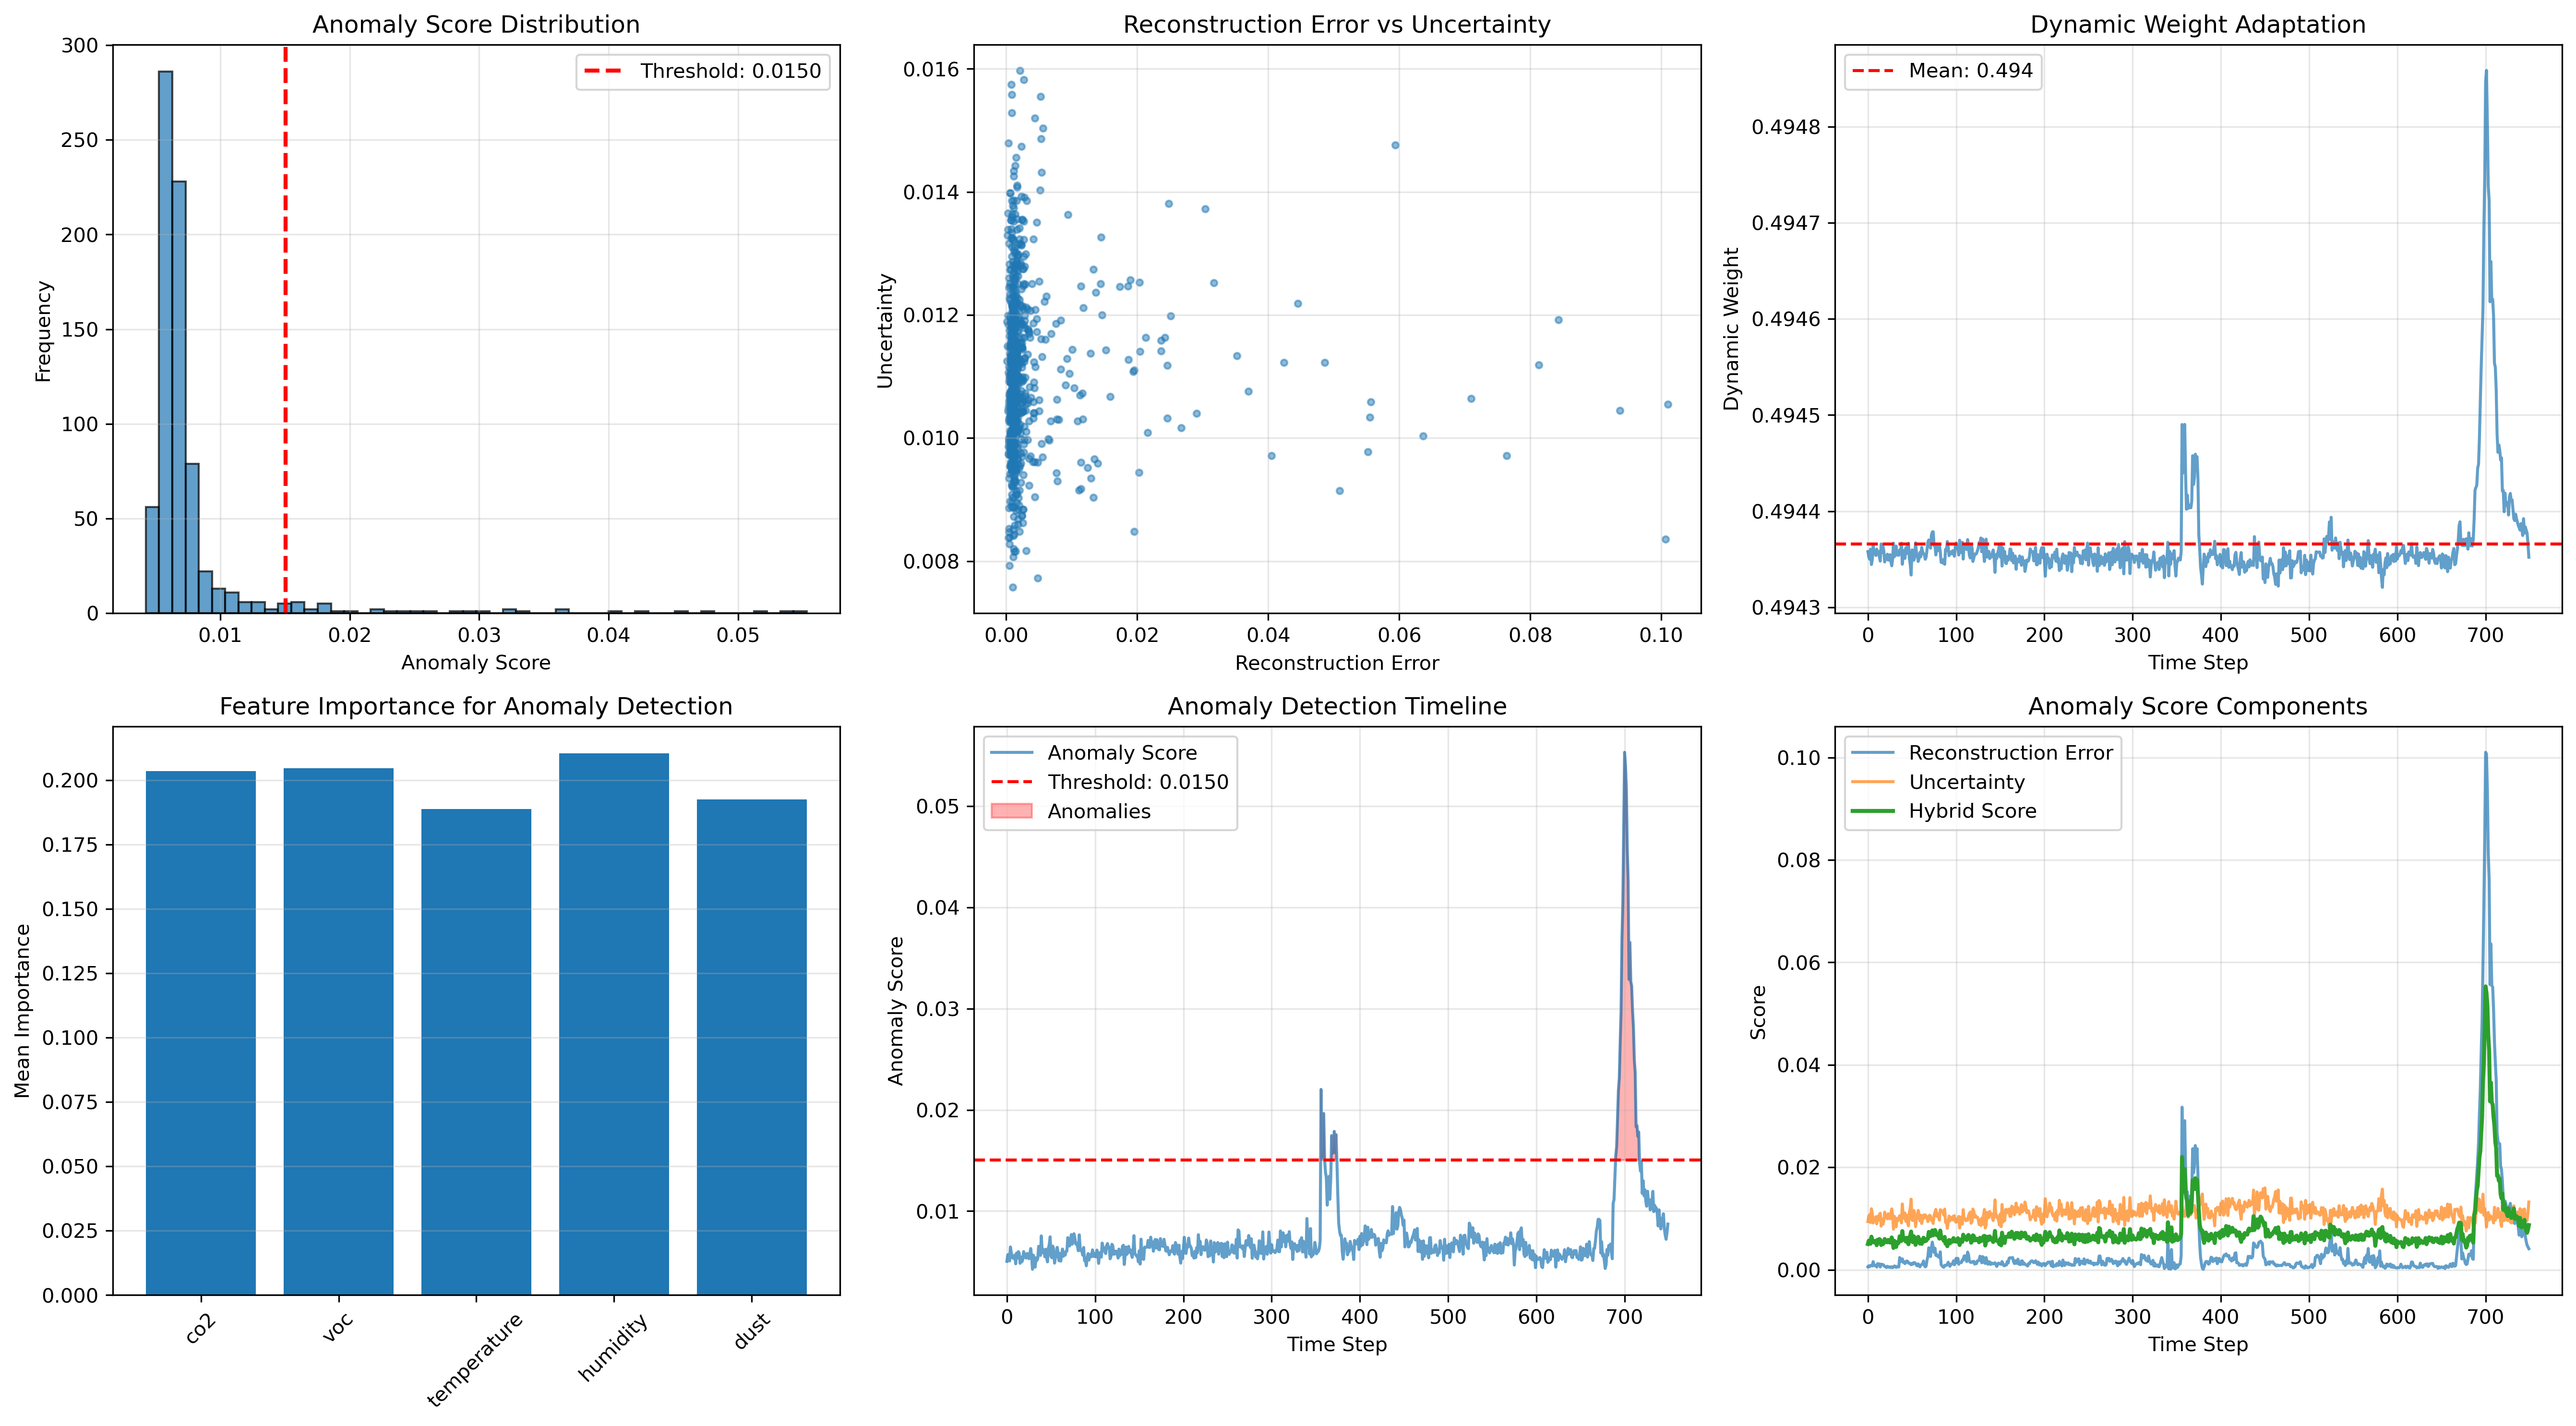
\includegraphics[width=0.95\linewidth]{images/current_anomaly_analysis.png}
    }
    \caption{Anomaly analysis visualization showing anomaly-score distribution, reconstruction error versus uncertainty, dynamic weights, feature importance, anomaly timeline, and score components.}
    \label{fig:anomaly_analysis}
\end{figure}


\subsection{Computational Efficiency Analysis}
We analyzed the computational cost of the proposed framework to ensure practical deployability. Table \ref{table:computational_cost} presents the comparison of model parameters, training time, and inference speed.

\begin{table}[htbp]
\centering
\caption{Computational Efficiency Comparison}
\label{table:computational_cost}
\begin{tabular}{lccc}
\toprule
\textbf{Model} & \textbf{Parameters} & \textbf{Train Time (s/epoch)} & \textbf{Inference (ms/sample)} \\
\midrule
RNN & 45.2K & 12.3 & 0.8 \\
LSTM & 89.6K & 18.7 & 1.2 \\
GRU & 72.4K & 15.2 & 1.0 \\
TCN & 98.3K & 14.8 & 0.9 \\
TCN + MC & 98.3K & 14.8 & 1.1 \\
TCN + MC + AUAA & 105.8K & 16.2 & 1.3 \\
\textbf{Full Enhanced} & \textbf{110.2K} & \textbf{17.1} & \textbf{1.4} \\
\bottomrule
\end{tabular}
\end{table}

The proposed TCN-Stochastic Enhanced introduces additional parameters compared to the base TCN while enabling uncertainty quantification, adaptive anomaly scoring, and feature-level attribution. The computational overhead should be interpreted as the cost of added interpretability and uncertainty-aware scoring capabilities.

\subsection{Feature Values with Uncertainty}
Visual analysis of actual versus predicted values highlights the model's forecasting ability and uncertainty quantification. The base TCN-Stochastic model achieves the best raw reconstruction metrics, while the enhanced model provides additional uncertainty and attribution outputs. The prediction plots should therefore be interpreted as qualitative diagnostics for temporal behavior rather than evidence that the enhanced model reduces raw MSE.

\begin{figure}[H]
    \centering
    \subfloat[]{
        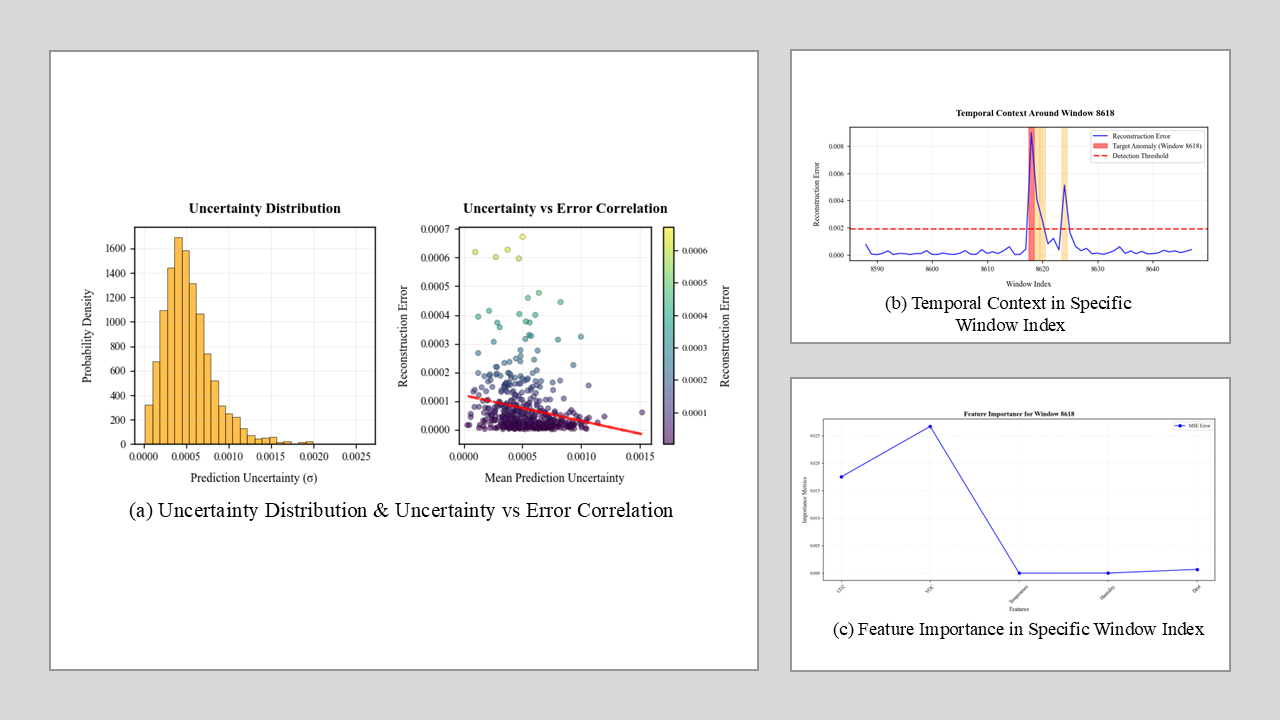
\includegraphics[width=0.9\linewidth]{images/uncertainty ad - window index.png}
    }
    \caption{The visualization of uncertainty, and the feature importance in specific windows.}
    \label{fig:uncertainty_windowidx}
\end{figure}

Figure \ref{fig:uncertainty_windowidx} shows how the TCN-Stochastic model assigns predictive confidence across temporal windows. The enhanced model's mean dynamic weight is 0.4944 with a narrow range from 0.4943 to 0.4949, indicating a slightly uncertainty-focused scoring balance. Mean feature attribution is distributed across the five sensors, with humidity contributing the largest share (21.0\%), followed by VOC (20.5\%), CO\textsubscript{2} (20.4\%), dust (19.2\%), and temperature (18.9\%).

\subsection{Anomaly Detection Analysis}
The TCN-Stochastic model detects anomalies by leveraging reconstruction errors and uncertainty. Figure \ref{fig:anomaly_analysis} shows the evaluation results for 750 validation windows. The base TCN-Stochastic model uses a 95th-percentile threshold of 0.001803 and detects 38 anomalies (5.07\%). The enhanced model uses an adaptive threshold of 0.015033 and also detects 38 anomalies (5.07\%). The figure presents score distributions, dynamic weights, feature importances, and anomaly timelines.

\subsection{Threshold Selection Analysis}
We compared the thresholding behavior of both models. Table \ref{table:threshold_comparison} presents the resulting thresholds and detection counts for the base and enhanced models.

\begin{table}[htbp]
\centering
\caption{Threshold Selection Results Generated by the Updated Source Code}
\label{table:threshold_comparison}
\begin{tabular}{lcccc}
\toprule
\textbf{Model} & \textbf{Method} & \textbf{Threshold} & \textbf{Detected} & \textbf{Ratio} \\
\midrule
TCN-Stochastic & Percentile (95\%) & 0.001803 & 38 & 5.07\% \\
TCN-Stochastic Enhanced & Adaptive & 0.015033 & 38 & 5.07\% \\
\bottomrule
\end{tabular}
\end{table}


The percentile-based threshold serves as a simple baseline, while the adaptive threshold is used by the enhanced model to combine reconstruction error with uncertainty-aware scoring. In the experiments, both methods flag 38 of 750 validation windows.

\subsection{Dynamic Weight Analysis}
The learned dynamic weights exhibit clear adaptation patterns across different operating conditions:

\textbf{Observed Operation (weights $\approx$ 0.494):} The learned weights remain close to 0.494, indicating a slightly uncertainty-focused balance between reconstruction error and uncertainty.

\textbf{High Variance Periods:} During periods of high sensor variance or potential degradation, this weighting mechanism is designed to shift emphasis toward uncertainty estimates, acknowledging reduced prediction reliability.

\textbf{Transition Regions:} The transition range is narrow (0.4943--0.4949), so the observed validation subset is best described as consistently uncertainty-focused rather than strongly regime-switching.

This adaptive behavior addresses the concern about sensor-specific challenges by enabling context-sensitive anomaly detection.
